% Homework #5
% COSC552 HCI
%
% Byron Heads
% E00062946

\documentclass[12pt]{report}

\usepackage{graphics}
\usepackage{hyperref, wasysym}
\usepackage{listings}
\usepackage{colortbl}
\definecolor{grey}{rgb}{0.8,0.8,0.8}


\title{Homework Set 5 \\
    COSC552 HCI}
\author{ Byron Heads \\
    E00062946 }
\date{\today}

\begin{document}
\maketitle

\chapter*{A}

The design of the search interface is based on a mix between free-form and defined searching.  The user is able to search for a keyword or phrase in the database, or they can limit the search to a single category.  This allows a user to do complex searches without having to learn complicated search syntax and reduces the complexity of the program.  This can reduce the program's development time.

\begin{figure}[h!]
\center{\resizebox{\columnwidth}{!}{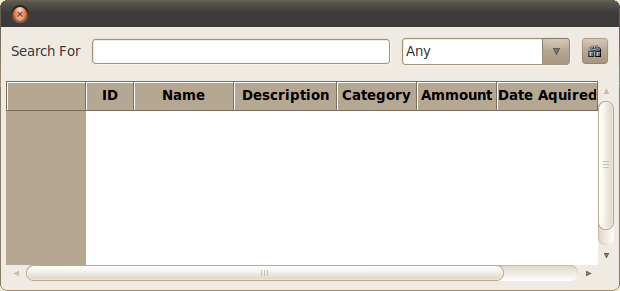
\includegraphics{ss1.png}}}
\caption{The search window.}
\end{figure}

The user can enter the keyword they want to search for in the first textbox and then select which category they would like to search.  The default category ``Any'' searches the entire database.

\begin{figure}[h!]
\center{\resizebox{\columnwidth}{!}{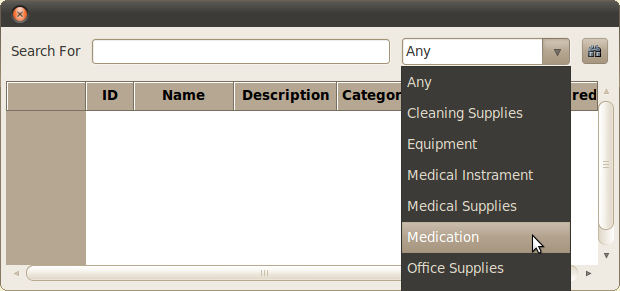
\includegraphics{ss2.png}}}
\caption{The category menu shows the top categories in the database.  The number of categories shown is set in the configuration menu.  The top categories are determined by the number of items in a category and how often that category is searched.  The user can type in any category they want to search.}
\end{figure}

\chapter*{}

To run a search, the user enters the term or phrase to search, then selects the search category, and then presses the search button.  To speed up entry input, the user can hit the tab key to switch to the next control.  Pressing enter will run the search without having to click on the search button.  The user can use the up and down keys to cycle through the list of categories or they can type in the category they want to search.

\begin{figure}[h!]
\center{\resizebox{\columnwidth}{!}{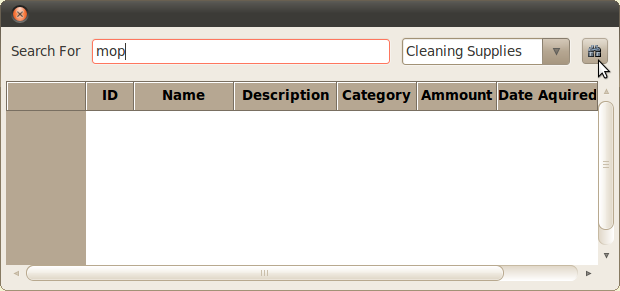
\includegraphics{ss3.png}}}
\caption{The user inputs a search to determine the number of mops in the office.}
\end{figure}

\begin{figure}[h!]
\center{\resizebox{\columnwidth}{!}{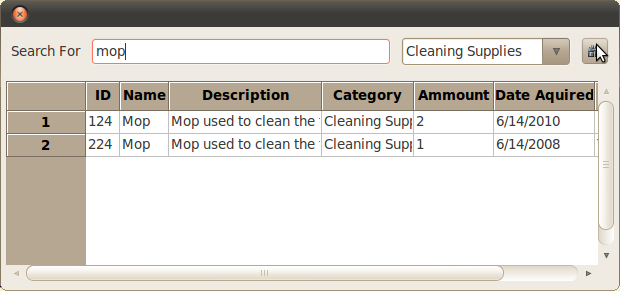
\includegraphics{ss4.png}}}
\caption{The search returns two entries for mop.}
\end{figure}

\begin{figure}[h!]
\center{\resizebox{\columnwidth}{!}{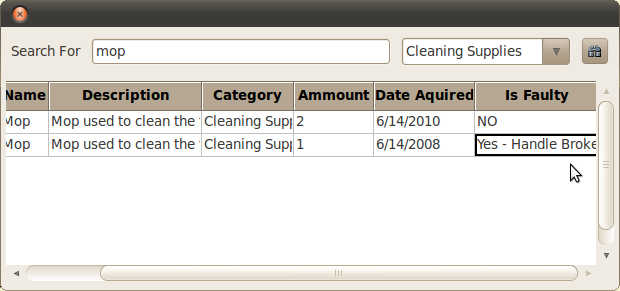
\includegraphics{ss6.png}}}
\caption{We see that the clinic has two good mops and one broken one.}
\end{figure}

\chapter*{}

The database search is carried out by converting the users search input into a SQL query.  By using categories, we can reduce the number of results returned to the user.  This makes reading the results easier for the user.  The search is done case-insensitive, and the keyword is searched against the item name, item description, item ID, and the faulty description.  For example, the search for mop in the sample images could possibly produce the following SQL:

\lstset{language=SQL}
\begin{lstlisting}
SELECT *
FROM "items"
WHERE ( "name" LIKE "mop" OR "description" LIKE "mop" OR 
    "id" LIKE "mop" OR "fault" LIKE "mop") 
    AND "category" LIKE "office supplies"
\end{lstlisting}

\chapter*{B}

Please answer the following questions to the best of your abilities.
\begin{description}
\item{\emph{SA}} - Strongly Agree
\item{\emph{A}} - Agree
\item{\emph{NO}} - No Opinion
\item{\emph{D}} - Disagree
\item{\emph{SD}} - Strongly Disagree
\end{description}

\noindent
\begin{tabular}{p{.65\linewidth} c c c c c }
 & SA & A & NO & D & SD \\ \hline 
The icons are easy to see and understand. & \Circle & \Circle & \Circle & \Circle & \Circle \\ \hline
\rowcolor{grey}I am often confused as how to do things. & \Circle & \Circle & \Circle & \Circle & \Circle \\ \hline
I can find the help menu. & \Circle & \Circle & \Circle & \Circle & \Circle \\ \hline
\rowcolor{grey}I often use the help menu. & \Circle & \Circle & \Circle & \Circle & \Circle \\ \hline
Using the program increase my stress. & \Circle & \Circle & \Circle & \Circle & \Circle \\ \hline
\rowcolor{grey}Inputting new items into the system is fast. & \Circle & \Circle & \Circle & \Circle & \Circle \\ \hline
I often only have to search once to find an item. & \Circle & \Circle & \Circle & \Circle & \Circle \\ \hline
\rowcolor{grey}It is difficult to find things in the menu. & \Circle & \Circle & \Circle & \Circle & \Circle \\ \hline
I often have to ask my coworkers for help. & \Circle & \Circle & \Circle & \Circle & \Circle \\ \hline
\rowcolor{grey}I am able to input a defective item. & \Circle & \Circle & \Circle & \Circle & \Circle \\ \hline
The item I am searching for is normally in the top ten results. & \Circle & \Circle & \Circle & \Circle & \Circle \\ \hline
\rowcolor{grey}I can add a new item into the system. & \Circle & \Circle & \Circle & \Circle & \Circle \\ \hline
I am comfortable with removing an item from the system. & \Circle & \Circle & \Circle & \Circle & \Circle \\ \hline
\rowcolor{grey}I worry about the program crashing. & \Circle & \Circle & \Circle & \Circle & \Circle \\ \hline
I can make a backup. & \Circle & \Circle & \Circle & \Circle & \Circle \\ \hline
\end{tabular}


\noindent
\begin{tabular}{p{.65\linewidth} c c c c c }
 & SA & A & NO & D & SD \\ \hline 
I often have to enter the same information twice.  & \Circle & \Circle & \Circle & \Circle & \Circle \\ \hline
\rowcolor{grey}It takes a long time to search for an item. & \Circle & \Circle & \Circle & \Circle & \Circle \\ \hline
The system uses the same terminology that we use in the office.  & \Circle & \Circle & \Circle & \Circle & \Circle \\ \hline
\rowcolor{grey}My disability makes it difficult to use the system. & \Circle & \Circle & \Circle & \Circle & \Circle \\ \hline
I often have to restart the program. & \Circle & \Circle & \Circle & \Circle & \Circle \\ \hline
\rowcolor{grey}I spend more time inputting data then searching. & \Circle & \Circle & \Circle & \Circle & \Circle \\ \hline
Most of the data fields are useless. & \Circle & \Circle & \Circle & \Circle & \Circle \\ \hline
\rowcolor{grey}I spend more then two hours a day on the system. & \Circle & \Circle & \Circle & \Circle & \Circle \\ \hline
The error messages are confusing. & \Circle & \Circle & \Circle & \Circle & \Circle \\ \hline
\rowcolor{grey}I prefer paper over the computer. & \Circle & \Circle & \Circle & \Circle & \Circle \\ \hline
I need to write down instructions to remember them. & \Circle & \Circle & \Circle & \Circle & \Circle \\ \hline
\rowcolor{grey}The screens look too similar. & \Circle & \Circle & \Circle & \Circle & \Circle \\ \hline
I speak out loud to remember how to do things. & \Circle & \Circle & \Circle & \Circle & \Circle \\ \hline
\rowcolor{grey}The menus are easy to navigate. & \Circle & \Circle & \Circle & \Circle & \Circle \\ \hline
It takes me several searches to find what I need. & \Circle & \Circle & \Circle & \Circle & \Circle \\ \hline
\rowcolor{grey}Removing items creates stress. & \Circle & \Circle & \Circle & \Circle & \Circle \\ \hline
I only use the system a few times a week. & \Circle & \Circle & \Circle & \Circle & \Circle \\ \hline
\rowcolor{grey}I am often waiting for the system to complete a task. & \Circle & \Circle & \Circle & \Circle & \Circle \\ \hline
I feel stress when using the system. & \Circle & \Circle & \Circle & \Circle & \Circle \\ \hline
\rowcolor{grey}I understand most buttons from the icon. & \Circle & \Circle & \Circle & \Circle & \Circle \\ \hline
I rarely look up how to do things. & \Circle & \Circle & \Circle & \Circle & \Circle \\ \hline
\rowcolor{grey}I want more data fields for the items in the database. & \Circle & \Circle & \Circle & \Circle & \Circle \\ \hline
The system does with I need it to do. & \Circle & \Circle & \Circle & \Circle & \Circle \\ \hline
\rowcolor{grey}It is easy to make a mistake. & \Circle & \Circle & \Circle & \Circle & \Circle \\ \hline
I like the help system. & \Circle & \Circle & \Circle & \Circle & \Circle \\ \hline

\end{tabular}

\subsubsection*{What about the system do you find confusing? }
\begin{tabular}{ p{\linewidth} } \ \\ \hline \ \\ \hline \ \\ \hline \ \\  \hline \end{tabular}


\subsubsection*{If I could change one thing, what would it be? }
\begin{tabular}{ p{\linewidth} } \ \\ \hline \ \\ \hline \ \\ \hline \ \\  \hline \end{tabular}

\subsubsection*{What about the system causes the most stress? }
\begin{tabular}{ p{\linewidth} } \ \\ \hline \ \\ \hline \ \\ \hline \ \\  \hline \end{tabular}

\subsubsection*{What about the system do you find confusing? }
\begin{tabular}{ p{\linewidth} } \ \\ \hline \ \\ \hline \ \\ \hline \ \\  \hline \end{tabular}

\subsubsection*{What about the system do you like the most? }
\begin{tabular}{ p{\linewidth} } \ \\ \hline \ \\ \hline \ \\ \hline \ \\  \hline \end{tabular}

\subsubsection*{Comments ? }
\begin{tabular}{ p{\linewidth} } \ \\ \hline \ \\ \hline \ \\ \hline \ \\  \hline \end{tabular}


\end{document}

